\section{Progettazione}
E' stato scelto \textit{Responsive Web Design} come strategia di progettazione, il sito infatti é in grado di adattarsi graficamente in modo automatico in base al dispositivo con il quale viene visualizzato. \\
Si è preferito usare  XHTML5  perché  ci  permette  di  usare  la  specifica  WAI-ARIA, discussa in seguito.

Il progetto è stato affrontato con un approccio top-down, individuando elementi generici da implementare e procedendo quindi con lo sviluppo di pagine e funzioni.


\subsection{Struttura delle pagine}
Sono di seguito riportati i differenti elementi della struttura delle pagine del sito.
\paragraph{Header}
L' header contiene il logo ed il nome del sito, due pulsanti per visualizzare la barra di ricerca delle birre ed accedere al profilo personale oltre ad una barra di navigazione con i riferimenti alle principali pagine del sito.\\
E' presente in tutte le pagine del sito.
\paragraph{Breadcrumb}
Sotto alla testata è situata la breadcrumb che permette all'utente di orientarsi visualizzando il percorso dalla homepage fino alla pagina corrente.\\
La breadcrumb non è visibile nelle pagine di avviso di contenuto non trovato e accesso negato in quanto sono pagine di eccezione.
\paragraph{Main}
La sezione Main visualizza il contenuto principale e caratterizzante della pagina.
\paragraph{Footer}
Al piede della pagina è situato il footer che riporta informazioni sul progetto e i relativi certificati di validazione.\\
\'E presente in tutte le pagine del sito.

\subsection{Struttura del sito}
L'index page del sito reindirizza alla pagina di verifica dell'età, mentre conduce direttamente alla homepage se nelle variabili di sessione è indicato che l'utente ha già eseguito la verifica ed è maggiorenne.\\
La verifica viene eseguita dalla pagina \textit{ageverification} stessa ed ogni altra pagina reindirizza a quest'ultima se rileva che nella sessione dell'utente non è presente la variabile che rappresenta l'avvenuta verifica.\\
Di seguito si riportano le pagine del sito e le rispettive caratteristiche.

\paragraph{Home}
L'\textit{homepage} è la pagina che viene mostrata all'utente dopo la verifica dell'età e contiene una lista di birre in offerta o consigliate dall'amministrazione.

\paragraph{Prodotti}
La pagina \textit{prodotti} visualizza tutte le birre disponibili nel database, suddivise in pagine.\\
La pagina viene inoltre utilizzata per visualizzare i risultati di una ricerca tramite la barra di ricerca.

\paragraph{Dettagli}
La pagina \textit{dettagli} visualizza informazioni complete e recensioni della birra scelta dalla pagina \textit{prodotti}.\\
Se l'utente ha effettuato l'accesso vengono visualizzati i controlli per aggiungere e rimuovere recensioni.

\paragraph{Contatti}
La pagina \textit{contatti} contiene una breve descrizione dell'azienda ed il contatto telefonico e di posta elettronica dell'azienda.

\paragraph{Spazio utente}
La registrazione e l'accesso degli utenti viene gestita dalle pagine \textit{login} e \textit{registrazione} mentre \textit{dettagliaccount} e \textit{modificadati} permettono la visualizzazione e la modifica dei dati del proprio profilo.

\paragraph{Avvisi}
Il tentativo di accesso ad aree vietate o a contenuti non disponibili viene notificato dalle pagine \textit{accessdenied} e \textit{notfound} mentre il risultato di query viene visualizzato in sezioni della pagina dalla quale viene eseguita l'operazione.\\
La pagina \textit{deleteaccount} avverte della corretta eliminazione dell'account e la pagina \textit{logout} si occupa di terminare la sessione e reindirizzare l'utente alla homepage.

\subsection{Attori}
Vengono di seguito elencati i possibili tipi di utenti che possono interagire con il sito.
\begin{itemize}
\item \textbf{Utente non abilitato:} Se l'utente non ha una sessione attiva o ha dichiarato di essere minorenne, ogni tentativo di accesso alle pagine del sito risulta in una ridirezione alla pagina di verifica dell'età, dalla quale può proseguire solo dopo aver confermato di essere maggiorenne;
\item \textbf{Utente maggiorenne e non loggato:} Un utente che ha dichiarato di essere maggiorenne e non è loggato nel sito ha accesso a tutte le pagine tranne quelle di gestione dell'account; il tentativo di accesso a quest'ultime verrà negato e segnalato da una pagina apposita.
L'utente può accedere alla pagina di registrazione attraverso il link \textit{Registrati} nella pagina login, raggiungibile dal tasto account situato nell'header.
Nelle pagine di dettagli delle birre saranno visualizzate le recensioni ma non ci sarà la possibilità di modificarle o aggiungerne di nuove;
\item \textbf{Utente maggiorenne e loggato:} Gli utenti che hanno effettuato l'accesso possono visitare tutte le pagine del sito ed hanno la possibilità di aggiungere ed eliminare le proprie recensioni.
Dalla pagina \textit{account} possono inoltre visualizzare e modificare i propri dati, effettuare il logout o eliminare l'account;
\item \textbf{Utente amministratore:} Un utente amministratore ha accesso a tutte le pagine del sito ed ha la possibilità di eliminare anche le recensioni degli altri utenti.
Un account deve essere eletto amministratore dagli operatori del database.
\end{itemize}

\newpage
\subsection{Accessibilitá}
Seguendo le linee guida per l'accessibilità del contenuto Web (WCAG 2.1), abbiamo modificato e aggiunto specifici elementi per rendere il nostro sito accessibile a tutti i nostri utenti, tra cui anche quelli che usano tecnologie assistive.   
\subsubsection{Percepibile}
\paragraph{Alternative testuali}
Tutti i contenuti non testuali presentati all'utente hanno un'alternativa testuale equivalente.
\paragraph{Adattabile}
Per la strategia seguita (\textit{Responsive Web Design} il sito non perde informazioni o struttura quando viene visualizzato in dispositivi diversi.
\paragraph{Distinguibile}
L'uso dei colori non è stato fatto solamente per presentazione ma si usano colori specifici che rappresentano emozioni, come per esempio l'uso del verde quando un'azione esegue con successo e l'uso del rosso quando succede il contrario.
La rappresentazione visiva del testo e immagini contenenti testo ha un rapporto di contrasto di almeno 7:1, che ci fa superare il test WCAG AAA.
\subsubsection{Utilizzabile}
I controlli sono correttamente assegnati ad una label e all'interno di form sono raggruppati da un tag \textit{fieldset}, descritto da un rispettivo tag \textit{legend}.\\
Tramite l'attributo \textit{tabindex} l'ordine di focus tramite tasto tab viene corretto o nascosto ad alcuni elementi di presentazione, come ad esempio le icone degli utenti delle recensioni, che sono quindi marcate con il valore \textit{presentation} dell'attributo \textit{role}.\\

I tag di heading sono stati utilizzati seguendo una corretta gerarchia ed in modo coerente per segnalare titoli e contenuti delle sezioni.\\
Nel sito sono assenti link circolari e sono presenti un \textit{hidden link} utile allo screen reader per saltare al contenuto della pagina ed un \textit{back-to-top-button} per tornare all'inizio della pagina.\\
\subsubsection{Comprensibile}
In aiuto ai sistemi di screen-reading sono inoltre segnalate le parole inglesi dagli attributi \textit{xml:lang} e \textit{lang}, le immagini principali sono dotate di un attributo \textit{alternative text} consono e i alcuni controlli marcati con l'attributo \textit{aria-label}.\\
I valori provenienti dai controlli, prima di essere processati lato server vengono validati e sanitizzati.
\subsubsection{Robusto}
Tutti i tag sono chiusi in modo corretto ed ogni pagina è caratterizzata da una lista adeguata di keyword.
\newpage
\subsection{Database}
Il sito sfrutta un database molto semplice, composto da tre tabelle:
\begin{itemize}
\item \textbf{Utenti:} raccoglie i dati anagrafici e di accesso di tutti gli utenti registrati al sito. \'E stata implementato un campo \textit{admin\textunderscore flag} che viene posto a \textit{TRUE} nel caso in cui l'account sia amministratore; la chiave primaria é un id auto-incrementate e \textit{username} é chiave univoca, così da impedire la registrazione al sito di più utenti con lo stesso username. Abbiamo deciso di non memorizzare la data di nascita nel database in quanto un utente che visita il sito deve aver dichiarato precedentemente di essere maggiorenne, un campo \textit{data\textunderscore nascita} per gli utenti non verrebbe quindi utilizzato e risulterebbe superfluo;
\item \textbf{Birre:} raccoglie i dati delle birre presenti nel sito. La chiave primaria é un id auto-incrementante, mentre il nome é chiave univoca, così da impedire l'inserimento di più birre con lo stesso nome;
\item \textbf{Recensioni:} raccoglie le recensioni delle birre (testo e voto) lasciate dagli utenti. La chiave primaria é un id auto-incrementante, ed essendo l'unica chiave un utente può lasciare più recensioni della stessa birra. Il campo \textit{utente} é chiave esterna riferita al campo \textit{id} della tabella \textit{Utenti} mentre il campo \textit{birra} é la chiave esterna riferita al campo \textit{id} della tabella \textit{Birre}.
\end{itemize}
Il database é normalizzato.
\begin{figure}[H]
	\centering
	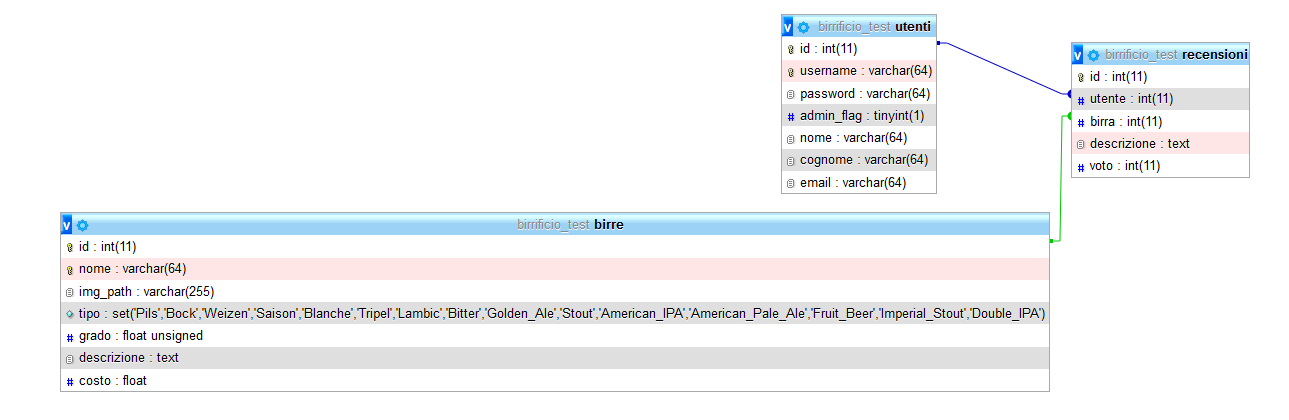
\includegraphics[width=16cm]{utility/db.png}
	\caption{UML database}
\end{figure}


